\documentclass{extbook}[14pt]
\usepackage{multicol, enumerate, enumitem, hyperref, color, soul, setspace, parskip, fancyhdr, amssymb, amsthm, amsmath, latexsym, units, mathtools}
\everymath{\displaystyle}
\usepackage[headsep=0.5cm,headheight=0cm, left=1 in,right= 1 in,top= 1 in,bottom= 1 in]{geometry}
\usepackage{dashrule}  % Package to use the command below to create lines between items
\newcommand{\litem}[1]{\item #1

\rule{\textwidth}{0.4pt}}
\pagestyle{fancy}
\lhead{}
\chead{Answer Key for Progress Quiz 6 Version C}
\rhead{}
\lfoot{1430-1829}
\cfoot{}
\rfoot{test}
\begin{document}
\textbf{This key should allow you to understand why you choose the option you did (beyond just getting a question right or wrong). \href{https://xronos.clas.ufl.edu/mac1105spring2020/courseDescriptionAndMisc/Exams/LearningFromResults}{More instructions on how to use this key can be found here}.}

\textbf{If you have a suggestion to make the keys better, \href{https://forms.gle/CZkbZmPbC9XALEE88}{please fill out the short survey here}.}

\textit{Note: This key is auto-generated and may contain issues and/or errors. The keys are reviewed after each exam to ensure grading is done accurately. If there are issues (like duplicate options), they are noted in the offline gradebook. The keys are a work-in-progress to give students as many resources to improve as possible.}

\rule{\textwidth}{0.4pt}

\begin{enumerate}\litem{
Construct the lowest-degree polynomial given the zeros below. Then, choose the intervals that contain the coefficients of the polynomial in the form $x^3+bx^2+cx+d$.
\[ -3 + 2 i \text{ and } -3 \]The solution is \( x^{3} +9 x^{2} +31 x + 39 \), which is option B.\begin{enumerate}[label=\Alph*.]
\item \( b \in [-5, 4], c \in [5.6, 7.3], \text{ and } d \in [0, 15] \)

$x^{3} + x^{2} +6 x + 9$, which corresponds to multiplying out $(x + 3)(x + 3)$.
\item \( b \in [7, 14], c \in [30.7, 35.8], \text{ and } d \in [32, 45] \)

* $x^{3} +9 x^{2} +31 x + 39$, which is the correct option.
\item \( b \in [-10, -6], c \in [30.7, 35.8], \text{ and } d \in [-46, -38] \)

$x^{3} -9 x^{2} +31 x -39$, which corresponds to multiplying out $(x-(-3 + 2 i))(x-(-3 - 2 i))(x -3)$.
\item \( b \in [-5, 4], c \in [-1.3, 3.2], \text{ and } d \in [-6, -3] \)

$x^{3} + x^{2} +x -6$, which corresponds to multiplying out $(x -2)(x + 3)$.
\item \( \text{None of the above.} \)

This corresponds to making an unanticipated error or not understanding how to use nonreal complex numbers to create the lowest-degree polynomial. If you chose this and are not sure what you did wrong, please contact the coordinator for help.
\end{enumerate}

\textbf{General Comment:} Remember that the conjugate of $a+bi$ is $a-bi$. Since these zeros always come in pairs, we need to multiply out $(x-(-3 + 2 i))(x-(-3 - 2 i))(x-(-3))$.
}
\litem{
Describe the end behavior of the polynomial below.
\[ f(x) = -9(x + 3)^{2}(x - 3)^{3}(x + 7)^{5}(x - 7)^{5} \]The solution is the graph below, which is option A.
\begin{center}
    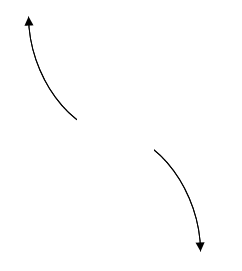
\includegraphics[width=0.3\textwidth]{../Figures/polyEndBehaviorCopyAC.png}
\end{center}\begin{enumerate}[label=\Alph*.]
\begin{multicols}{2}
\item 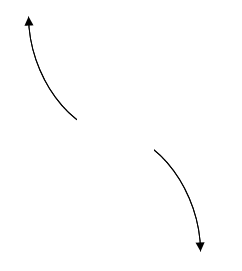
\includegraphics[width = 0.3\textwidth]{../Figures/polyEndBehaviorCopyAC.png}
\item 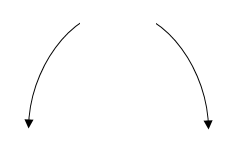
\includegraphics[width = 0.3\textwidth]{../Figures/polyEndBehaviorCopyBC.png}
\item 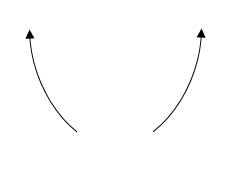
\includegraphics[width = 0.3\textwidth]{../Figures/polyEndBehaviorCopyCC.png}
\item 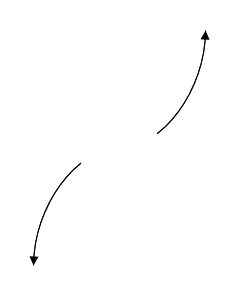
\includegraphics[width = 0.3\textwidth]{../Figures/polyEndBehaviorCopyDC.png}
\end{multicols}\item None of the above.\end{enumerate}
\textbf{General Comment:} Remember that end behavior is determined by the leading coefficient AND whether the \textbf{sum} of the multiplicities is positive or negative.
}
\litem{
Describe the zero behavior of the zero $x = 7$ of the polynomial below.
\[ f(x) = -6(x - 4)^{7}(x + 4)^{4}(x + 7)^{7}(x - 7)^{2} \]The solution is the graph below, which is option B.
\begin{center}
    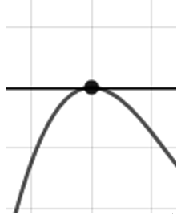
\includegraphics[width=0.3\textwidth]{../Figures/polyZeroBehaviorBC.png}
\end{center}\begin{enumerate}[label=\Alph*.]
\begin{multicols}{2}
\item 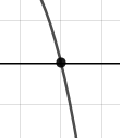
\includegraphics[width = 0.3\textwidth]{../Figures/polyZeroBehaviorAC.png}
\item 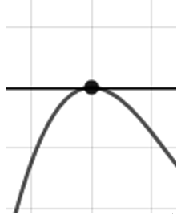
\includegraphics[width = 0.3\textwidth]{../Figures/polyZeroBehaviorBC.png}
\item 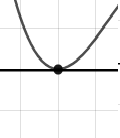
\includegraphics[width = 0.3\textwidth]{../Figures/polyZeroBehaviorCC.png}
\item 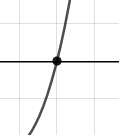
\includegraphics[width = 0.3\textwidth]{../Figures/polyZeroBehaviorDC.png}
\end{multicols}\item None of the above.\end{enumerate}
\textbf{General Comment:} You will need to sketch the entire graph, then zoom in on the zero the question asks about.
}
\litem{
Construct the lowest-degree polynomial given the zeros below. Then, choose the intervals that contain the coefficients of the polynomial in the form $ax^3+bx^2+cx+d$.
\[ \frac{5}{4}, -5, \text{ and } \frac{-4}{5} \]The solution is \( 20x^{3} +91 x^{2} -65 x -100 \), which is option A.\begin{enumerate}[label=\Alph*.]
\item \( a \in [17, 27], b \in [86, 92], c \in [-71, -61], \text{ and } d \in [-100, -98] \)

* $20x^{3} +91 x^{2} -65 x -100$, which is the correct option.
\item \( a \in [17, 27], b \in [-59, -53], c \in [-192, -178], \text{ and } d \in [-100, -98] \)

$20x^{3} -59 x^{2} -185 x -100$, which corresponds to multiplying out $(4x + 5)(x -5)(5x + 4)$.
\item \( a \in [17, 27], b \in [86, 92], c \in [-71, -61], \text{ and } d \in [98, 103] \)

$20x^{3} +91 x^{2} -65 x + 100$, which corresponds to multiplying everything correctly except the constant term.
\item \( a \in [17, 27], b \in [140, 144], c \in [220, 226], \text{ and } d \in [98, 103] \)

$20x^{3} +141 x^{2} +225 x + 100$, which corresponds to multiplying out $(4x + 5)(x + 5)(5x + 4)$.
\item \( a \in [17, 27], b \in [-98, -90], c \in [-71, -61], \text{ and } d \in [98, 103] \)

$20x^{3} -91 x^{2} -65 x + 100$, which corresponds to multiplying out $(4x + 5)(x -5)(5x -4)$.
\end{enumerate}

\textbf{General Comment:} To construct the lowest-degree polynomial, you want to multiply out $(4x -5)(x + 5)(5x + 4)$
}
\litem{
Construct the lowest-degree polynomial given the zeros below. Then, choose the intervals that contain the coefficients of the polynomial in the form $ax^3+bx^2+cx+d$.
\[ \frac{3}{4}, \frac{1}{2}, \text{ and } 6 \]The solution is \( 8x^{3} -58 x^{2} +63 x -18 \), which is option A.\begin{enumerate}[label=\Alph*.]
\item \( a \in [8, 11], b \in [-65, -57], c \in [61, 72], \text{ and } d \in [-19, -16] \)

* $8x^{3} -58 x^{2} +63 x -18$, which is the correct option.
\item \( a \in [8, 11], b \in [-40, -35], c \in [-61, -55], \text{ and } d \in [-19, -16] \)

$8x^{3} -38 x^{2} -57 x -18$, which corresponds to multiplying out $(4x + 3)(2x + 1)(x -6)$.
\item \( a \in [8, 11], b \in [51, 60], c \in [61, 72], \text{ and } d \in [17, 19] \)

$8x^{3} +58 x^{2} +63 x + 18$, which corresponds to multiplying out $(4x + 3)(2x + 1)(x + 6)$.
\item \( a \in [8, 11], b \in [-65, -57], c \in [61, 72], \text{ and } d \in [17, 19] \)

$8x^{3} -58 x^{2} +63 x + 18$, which corresponds to multiplying everything correctly except the constant term.
\item \( a \in [8, 11], b \in [-48, -40], c \in [-17, -9], \text{ and } d \in [17, 19] \)

$8x^{3} -46 x^{2} -15 x + 18$, which corresponds to multiplying out $(4x + 3)(2x -1)(x -6)$.
\end{enumerate}

\textbf{General Comment:} To construct the lowest-degree polynomial, you want to multiply out $(4x -3)(2x -1)(x -6)$
}
\litem{
Which of the following equations \textit{could} be of the graph presented below?

\begin{center}
    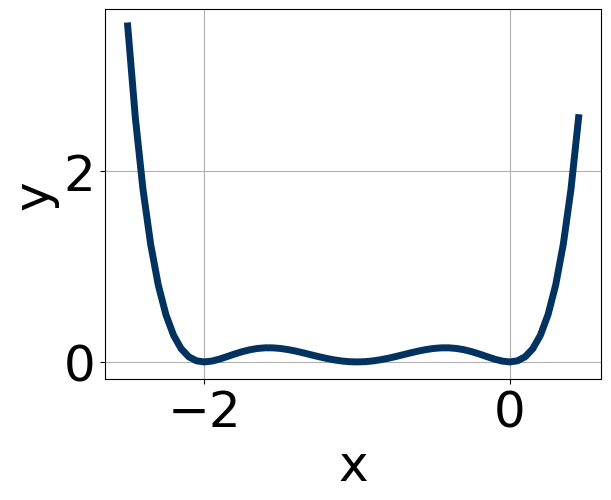
\includegraphics[width=0.5\textwidth]{../Figures/polyGraphToFunctionCopyC.png}
\end{center}


The solution is \( -13(x - 2)^{10} (x - 1)^{9} (x + 1)^{7} \), which is option A.\begin{enumerate}[label=\Alph*.]
\item \( -13(x - 2)^{10} (x - 1)^{9} (x + 1)^{7} \)

* This is the correct option.
\item \( -5(x - 2)^{11} (x - 1)^{10} (x + 1)^{5} \)

The factor $2$ should have an even power and the factor $1$ should have an odd power.
\item \( 3(x - 2)^{8} (x - 1)^{7} (x + 1)^{10} \)

The factor $(x + 1)$ should have an odd power and the leading coefficient should be the opposite sign.
\item \( -10(x - 2)^{6} (x - 1)^{6} (x + 1)^{9} \)

The factor $(x - 1)$ should have an odd power.
\item \( 6(x - 2)^{10} (x - 1)^{7} (x + 1)^{9} \)

This corresponds to the leading coefficient being the opposite value than it should be.
\end{enumerate}

\textbf{General Comment:} General Comments: Draw the x-axis to determine which zeros are touching (and so have even multiplicity) or cross (and have odd multiplicity).
}
\litem{
Which of the following equations \textit{could} be of the graph presented below?

\begin{center}
    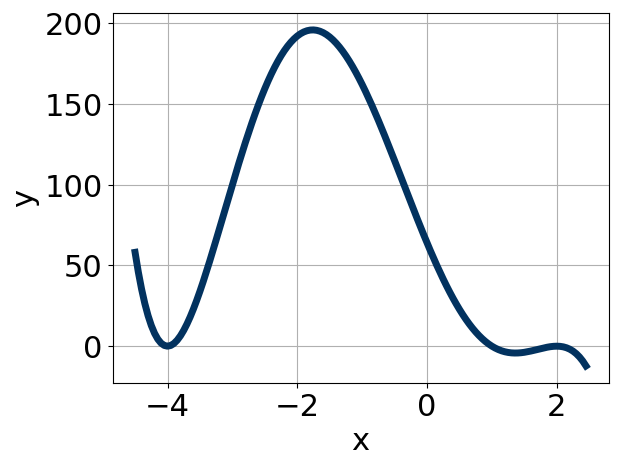
\includegraphics[width=0.5\textwidth]{../Figures/polyGraphToFunctionC.png}
\end{center}


The solution is \( -17(x + 3)^{4} (x + 4)^{6} (x - 1)^{10} \), which is option E.\begin{enumerate}[label=\Alph*.]
\item \( -15(x + 3)^{8} (x + 4)^{5} (x - 1)^{9} \)

The factors $(x + 4)$ and $(x - 1)$ should both have even powers.
\item \( 11(x + 3)^{10} (x + 4)^{6} (x - 1)^{9} \)

The factor $(x - 1)$ should have an even power and the leading coefficient should be the opposite sign.
\item \( -11(x + 3)^{6} (x + 4)^{4} (x - 1)^{11} \)

The factor $(x - 1)$ should have an even power.
\item \( 16(x + 3)^{4} (x + 4)^{8} (x - 1)^{4} \)

This corresponds to the leading coefficient being the opposite value than it should be.
\item \( -17(x + 3)^{4} (x + 4)^{6} (x - 1)^{10} \)

* This is the correct option.
\end{enumerate}

\textbf{General Comment:} General Comments: Draw the x-axis to determine which zeros are touching (and so have even multiplicity) or cross (and have odd multiplicity).
}
\litem{
Describe the zero behavior of the zero $x = 4$ of the polynomial below.
\[ f(x) = -2(x - 3)^{4}(x + 3)^{2}(x - 4)^{9}(x + 4)^{8} \]The solution is the graph below, which is option A.
\begin{center}
    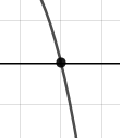
\includegraphics[width=0.3\textwidth]{../Figures/polyZeroBehaviorCopyAC.png}
\end{center}\begin{enumerate}[label=\Alph*.]
\begin{multicols}{2}
\item 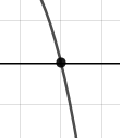
\includegraphics[width = 0.3\textwidth]{../Figures/polyZeroBehaviorCopyAC.png}
\item 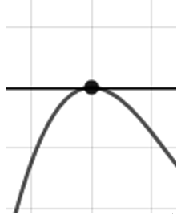
\includegraphics[width = 0.3\textwidth]{../Figures/polyZeroBehaviorCopyBC.png}
\item 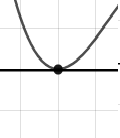
\includegraphics[width = 0.3\textwidth]{../Figures/polyZeroBehaviorCopyCC.png}
\item 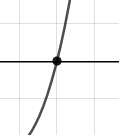
\includegraphics[width = 0.3\textwidth]{../Figures/polyZeroBehaviorCopyDC.png}
\end{multicols}\item None of the above.\end{enumerate}
\textbf{General Comment:} You will need to sketch the entire graph, then zoom in on the zero the question asks about.
}
\litem{
Construct the lowest-degree polynomial given the zeros below. Then, choose the intervals that contain the coefficients of the polynomial in the form $x^3+bx^2+cx+d$.
\[ -5 - 3 i \text{ and } 3 \]The solution is \( x^{3} +7 x^{2} +4 x -102 \), which is option A.\begin{enumerate}[label=\Alph*.]
\item \( b \in [6, 12], c \in [3.05, 4.75], \text{ and } d \in [-104, -101] \)

* $x^{3} +7 x^{2} +4 x -102$, which is the correct option.
\item \( b \in [-11, -5], c \in [3.05, 4.75], \text{ and } d \in [101, 108] \)

$x^{3} -7 x^{2} +4 x + 102$, which corresponds to multiplying out $(x-(-5 - 3 i))(x-(-5 + 3 i))(x + 3)$.
\item \( b \in [-6, 4], c \in [-0.86, 0.21], \text{ and } d \in [-14, -3] \)

$x^{3} + x^{2} +0 x -9$, which corresponds to multiplying out $(x + 3)(x -3)$.
\item \( b \in [-6, 4], c \in [1.77, 2.48], \text{ and } d \in [-17, -13] \)

$x^{3} + x^{2} +2 x -15$, which corresponds to multiplying out $(x + 5)(x -3)$.
\item \( \text{None of the above.} \)

This corresponds to making an unanticipated error or not understanding how to use nonreal complex numbers to create the lowest-degree polynomial. If you chose this and are not sure what you did wrong, please contact the coordinator for help.
\end{enumerate}

\textbf{General Comment:} Remember that the conjugate of $a+bi$ is $a-bi$. Since these zeros always come in pairs, we need to multiply out $(x-(-5 - 3 i))(x-(-5 + 3 i))(x-(3))$.
}
\litem{
Describe the end behavior of the polynomial below.
\[ f(x) = -5(x - 6)^{3}(x + 6)^{6}(x + 4)^{4}(x - 4)^{6} \]The solution is the graph below, which is option A.
\begin{center}
    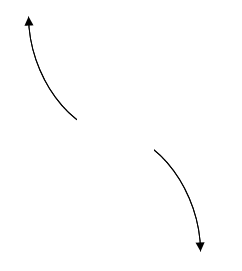
\includegraphics[width=0.3\textwidth]{../Figures/polyEndBehaviorAC.png}
\end{center}\begin{enumerate}[label=\Alph*.]
\begin{multicols}{2}
\item 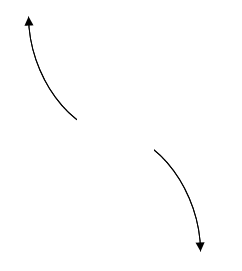
\includegraphics[width = 0.3\textwidth]{../Figures/polyEndBehaviorAC.png}
\item 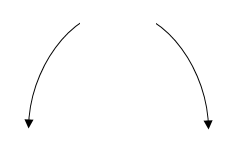
\includegraphics[width = 0.3\textwidth]{../Figures/polyEndBehaviorBC.png}
\item 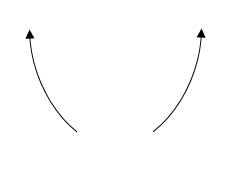
\includegraphics[width = 0.3\textwidth]{../Figures/polyEndBehaviorCC.png}
\item 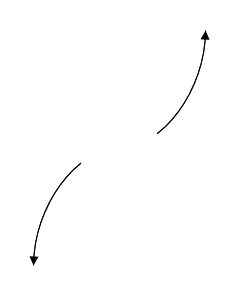
\includegraphics[width = 0.3\textwidth]{../Figures/polyEndBehaviorDC.png}
\end{multicols}\item None of the above.\end{enumerate}
\textbf{General Comment:} Remember that end behavior is determined by the leading coefficient AND whether the \textbf{sum} of the multiplicities is positive or negative.
}
\end{enumerate}

\end{document}